% CVPR 2026 Paper Template; see https://github.com/cvpr-org/author-kit

\documentclass[10pt,twocolumn,letterpaper]{article}

\usepackage{authblk}

%%%%%%%%% PAPER TYPE  - PLEASE UPDATE FOR FINAL VERSION
\usepackage{cvpr}                % To produce the CAMERA-READY version
% \usepackage[review]{cvpr}        % To produce the REVIEW version
%\usepackage[pagenumbers]{cvpr}    % To force page numbers, e.g. for an arXiv version
\usepackage{tikz}
\usepackage{standalone} % Required for including standalone .tex image files
\usepackage{float}
\usetikzlibrary{shapes, arrows.meta, positioning, calc, fit}

% Import additional packages in the preamble file, before hyperref
\input{preamble}

% It is strongly recommended to use hyperref, especially for the review version.
% hyperref with option pagebackref eases the reviewers' job.
% Please disable hyperref *only* if you encounter grave issues, 
% e.g. with the file validation for the camera-ready version.
%
% If you comment hyperref and then uncomment it, you should delete *.aux before re-running LaTeX.
% (Or just hit 'q' on the first LaTeX run, let it finish, and you should be clear).
\definecolor{cvprblue}{rgb}{0.21,0.49,0.74}
\usepackage[pagebackref,breaklinks,colorlinks,allcolors=cvprblue]{hyperref}

%%%%%%%%% PAPER ID  - PLEASE UPDATE
\def\paperID{*****} % *** Enter the Paper ID here
\def\confName{CVPR}
\def\confYear{2026}

%%%%%%%%% TITLE
\title{Semantic Correspondence}

%%%%%%%%% AUTHORS - PLEASE UPDATE
\author[1]{Luca Ostinelli}
\author[1]{Mostafa Kordi}
\author[1]{Zirui Luo}
\author[1]{Guoqiang Zhang}

\affil[1]{Politecnico di Torino, Torino, Italy}
\affil[ ]{\tt\small \{luca.ostinelli, s329702, s328249, s324461\}@studenti.polito.it}



\begin{document}
\maketitle
\begin{abstract}
Establishing pixel-level semantic correspondences across images with extreme variations in viewpoint, scale, and appearance remains a fundamental challenge in computer vision. This report systematically investigates the dense matching capabilities of modern Visual Foundation Models (VFMs)—specifically DINOv2, DINOv3, and the Segment Anything Model (SAM)—evaluated on the highly challenging SPair-71k benchmark. 

Our study follows a structured, multi-stage pipeline:
\begin{itemize}
    \item \textbf{Training-Free Baseline:} Zero-shot dense feature matching utilizing cosine similarity and standard argmax.
    \item \textbf{Light Fine-Tuning \& PEFT:} Task-specific adaptation of the latest ViT blocks, exploring efficient strategies like Low-Rank Adaptation (LoRA).
    \item \textbf{Inference Refinement:} Replacement of discrete argmax with Windowed Soft-Argmax to achieve sub-pixel accuracy and robustness against local noise.
\end{itemize}

By evaluating the Percentage of Correct Keypoints (PCK) across multiple precision thresholds, we provide a comprehensive analysis of the trade-offs between zero-shot generalization, fine-tuned accuracy, and computational efficiency.
\end{abstract}    
\section{Introduction}
\label{sec:intro}

\begin{figure}[ht]
    \centering
    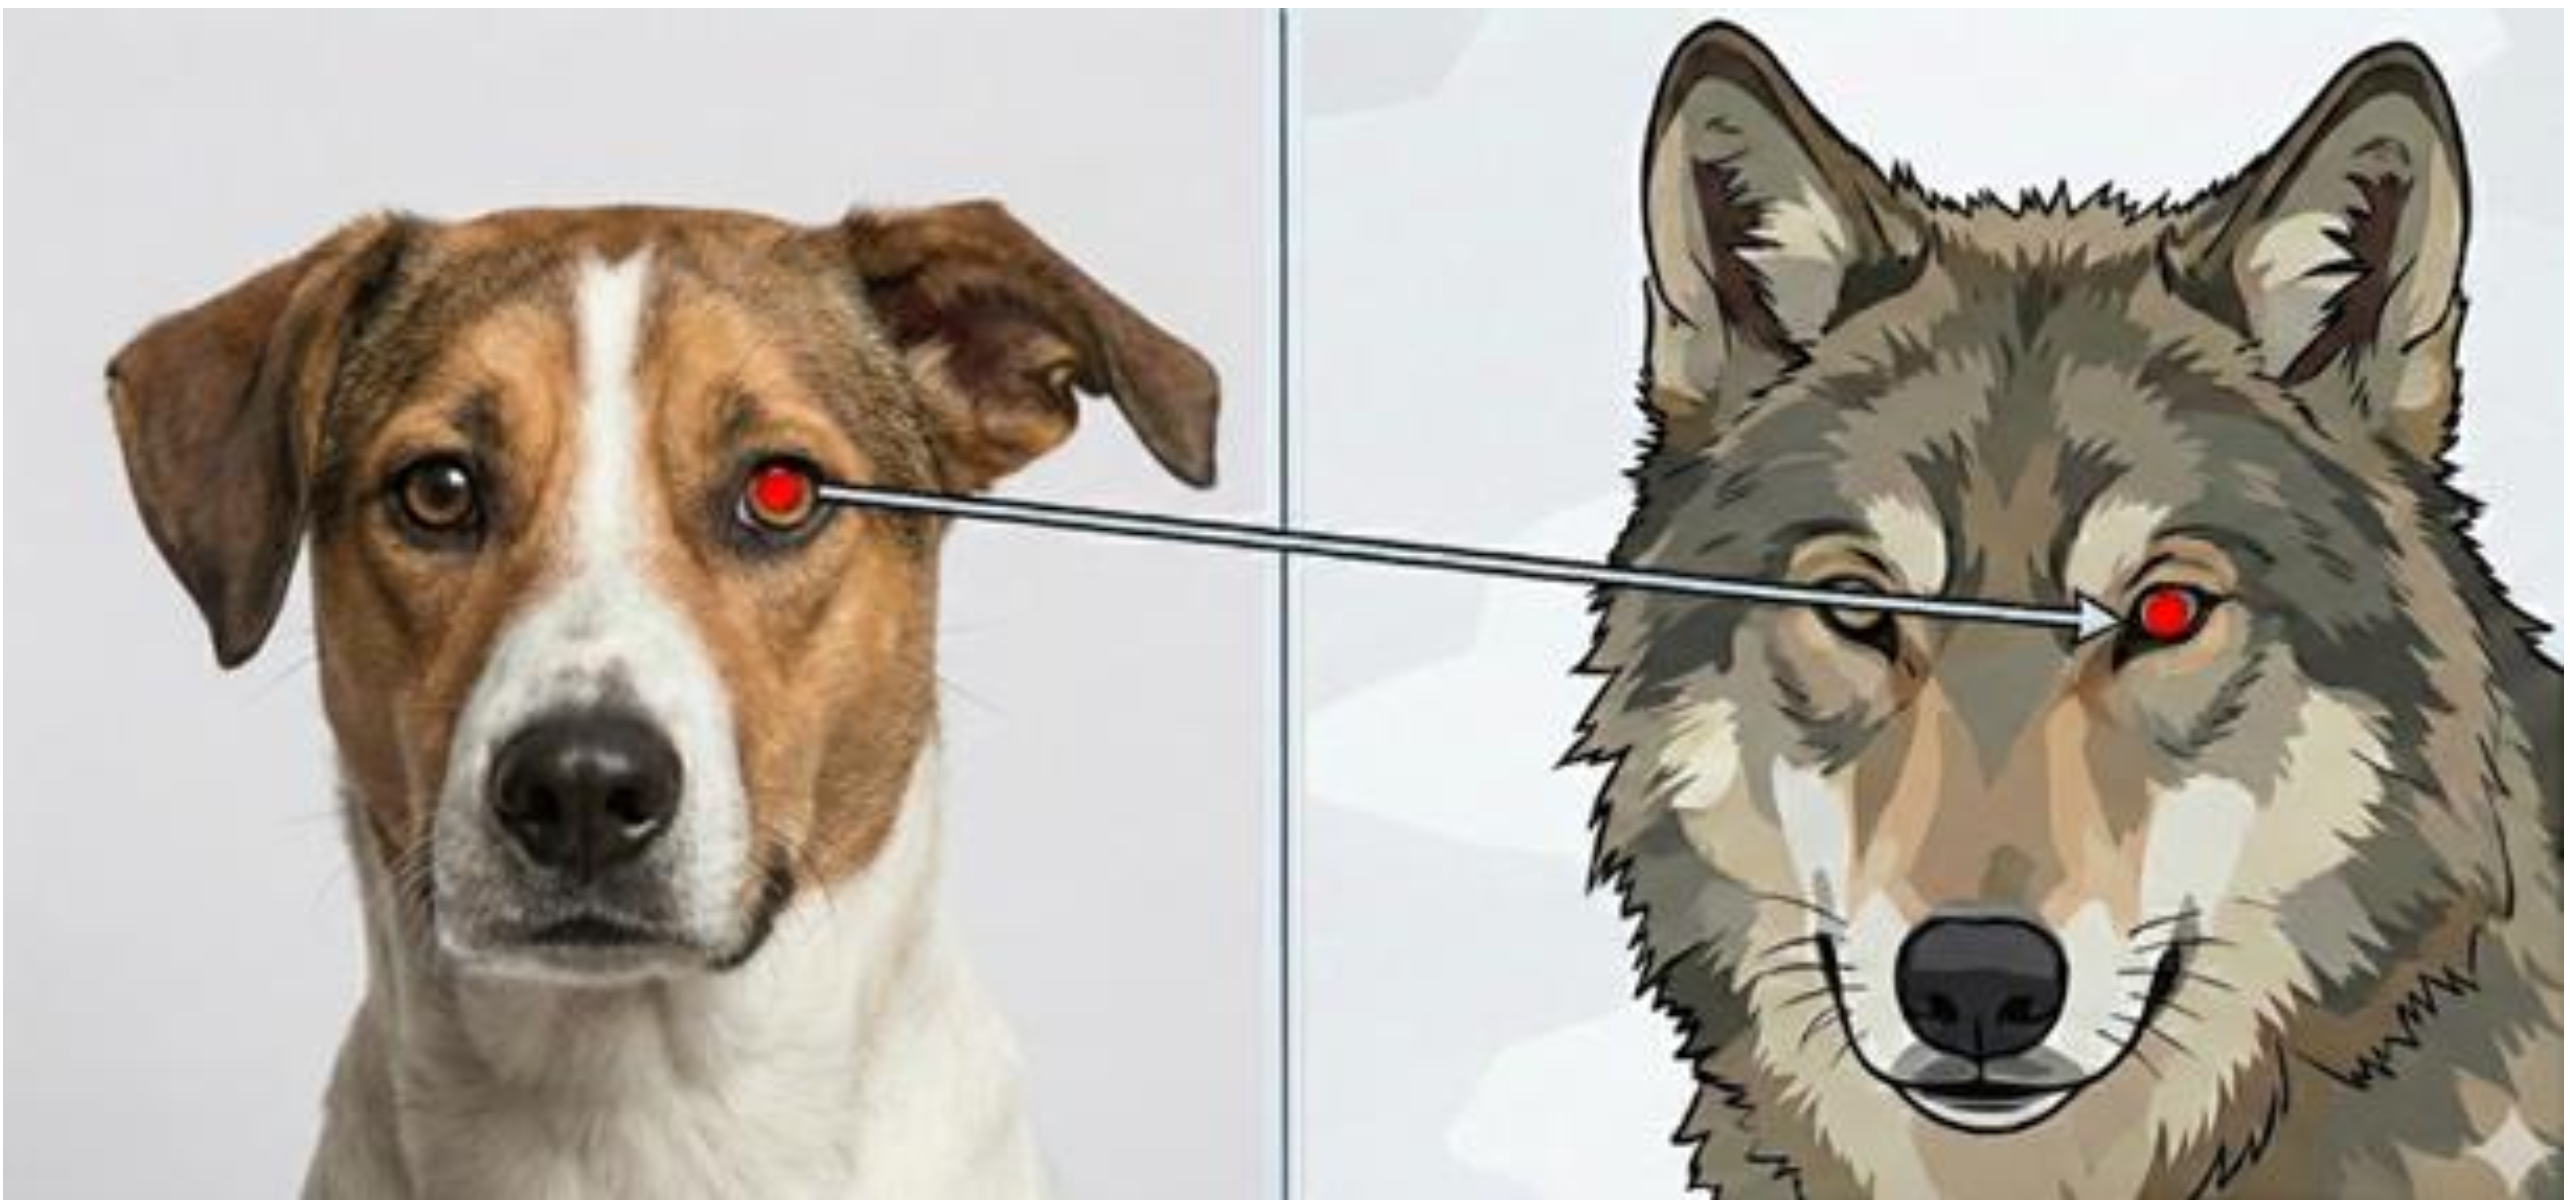
\includegraphics[width=\columnwidth]{img/teaser.png}
    \caption{Semantic correspondence across domains: matching the left eye of a dog in a photograph to the left eye of a wolf in an illustration.}
    \label{fig:teaser}
\end{figure}

Semantic correspondence is the complex task of finding pixel-level matches between semantically similar parts of objects across different images. Unlike standard geometric matching, which typically aligns different views of the exact same physical scene, semantic matching requires models to inherently understand object similarities despite drastic variations. Objects may appear in entirely different viewpoints, scales, or contexts, and the images themselves may originate from completely different visual domains, such as natural photographs versus artistic paintings. Furthermore, the system must accurately distinguish semantically similar but geometrically distinct parts, such as differentiating a left paw from a right paw.

Recent research demonstrates that large-scale Visual Foundation Models (VFMs) encompass rich internal representations that naturally support dense matching tasks. These representations emerge without explicit supervision, offering a highly effective starting point for semantic correspondence.

The primary goal of this project is to establish pixel-accurate semantic correspondences between a source image with annotated keypoints and a target image, leveraging features extracted from pre-trained visual encoders (DINOv2, DINOv3, and SAM). 

To systematically address and evaluate this task on the SPair-71k benchmark, the project is structured into four main stages:
\begin{itemize}
    \item \textbf{Training-Free Baseline:} Evaluating how well frozen features encode correspondence using cosine similarity and standard argmax.
    \item \textbf{Light Fine-Tuning:} Unfreezing and adapting the final layers of the backbone with keypoint supervision to enhance matching performance.
    \item \textbf{Prediction Refinement:} Replacing the discrete argmax operation with a Windowed Soft-Argmax to achieve sub-pixel accuracy and robustness against local noise.
    \item \textbf{Extension:} Exploring advanced strategies, specifically Parameter-Efficient Fine-Tuning via Low-Rank Adaptation (LoRA).
\end{itemize}
\section{Related Work}
\label{sec:related}

This section outlines the foundational literature and methodological advancements that form the basis of our project.

\paragraph{Semantic Correspondence and Benchmarks.}
The development of dense semantic correspondence models relies heavily on robust benchmarks. \textbf{SPair-71k}~\cite{min2019spair} serves as the standard dataset for this task, featuring extreme intra-class variations in scale, viewpoint, and occlusion levels. 

\begin{figure}[ht]
    \centering
    \includegraphics[width=\columnwidth]{img/spair_examples.png}
    \caption{Examples from the SPair-71k benchmark illustrating extreme intra-class variations in scale, viewpoint, and occlusion.}
    \label{fig:spair_dataset}
\end{figure}

To overcome the discretization limits inherent in standard matching pipelines evaluated on such benchmarks, recent approaches have introduced sub-pixel refinement techniques, notably the \textit{Windowed Soft-Argmax}~\cite{zhang2024telling}.

\paragraph{Visual Foundation Models (VFMs).}
Large-scale pre-trained models provide dense feature representations that are highly effective for zero-shot matching:
\begin{itemize}
    \item \textbf{DINO Family:} Leveraging the emergent properties of Vision Transformers (ViTs)~\cite{caron2021emerging}, \textbf{DINOv2}~\cite{oquab2023dinov2} and \textbf{DINOv3}~\cite{simeoni2025dinov3} extract highly robust, unsupervised semantic features.
    \item \textbf{Segment Anything Model (SAM):}~\cite{kirillov2023segment} Trained extensively on masks, SAM provides exceptional spatial and part-to-whole decomposition, acting as a structural complement to purely semantic models.
\end{itemize}

\paragraph{Diffusion Features.}
Alongside ViTs, intermediate features extracted from generative diffusion models (e.g., Stable Diffusion) exhibit emergent geometric correspondence capabilities~\cite{tang2023emergent}. These geometry-aware representations achieve state-of-the-art zero-shot performance when complementarily fused with DINO's semantic features~\cite{zhang2023tale}.

\paragraph{Parameter-Efficient Fine-Tuning (PEFT).}
To perform supervised adaptation (e.g., light fine-tuning) without updating the entire backbone, PEFT techniques are employed:
\begin{itemize}
    \item \textbf{LoRA}~\cite{hu2022lora}: Injects trainable low-rank matrices into the Transformer blocks to drastically reduce computational overhead.
    \item \textbf{AdaptFormer}~\cite{chen2022adaptformer} and \textbf{Adapters}~\cite{houlsby2019parameter}: Insert parallel or sequential trainable bottleneck modules to efficiently adapt pre-trained models to downstream tasks.
\end{itemize}

\begin{figure}[ht]
    \centering
    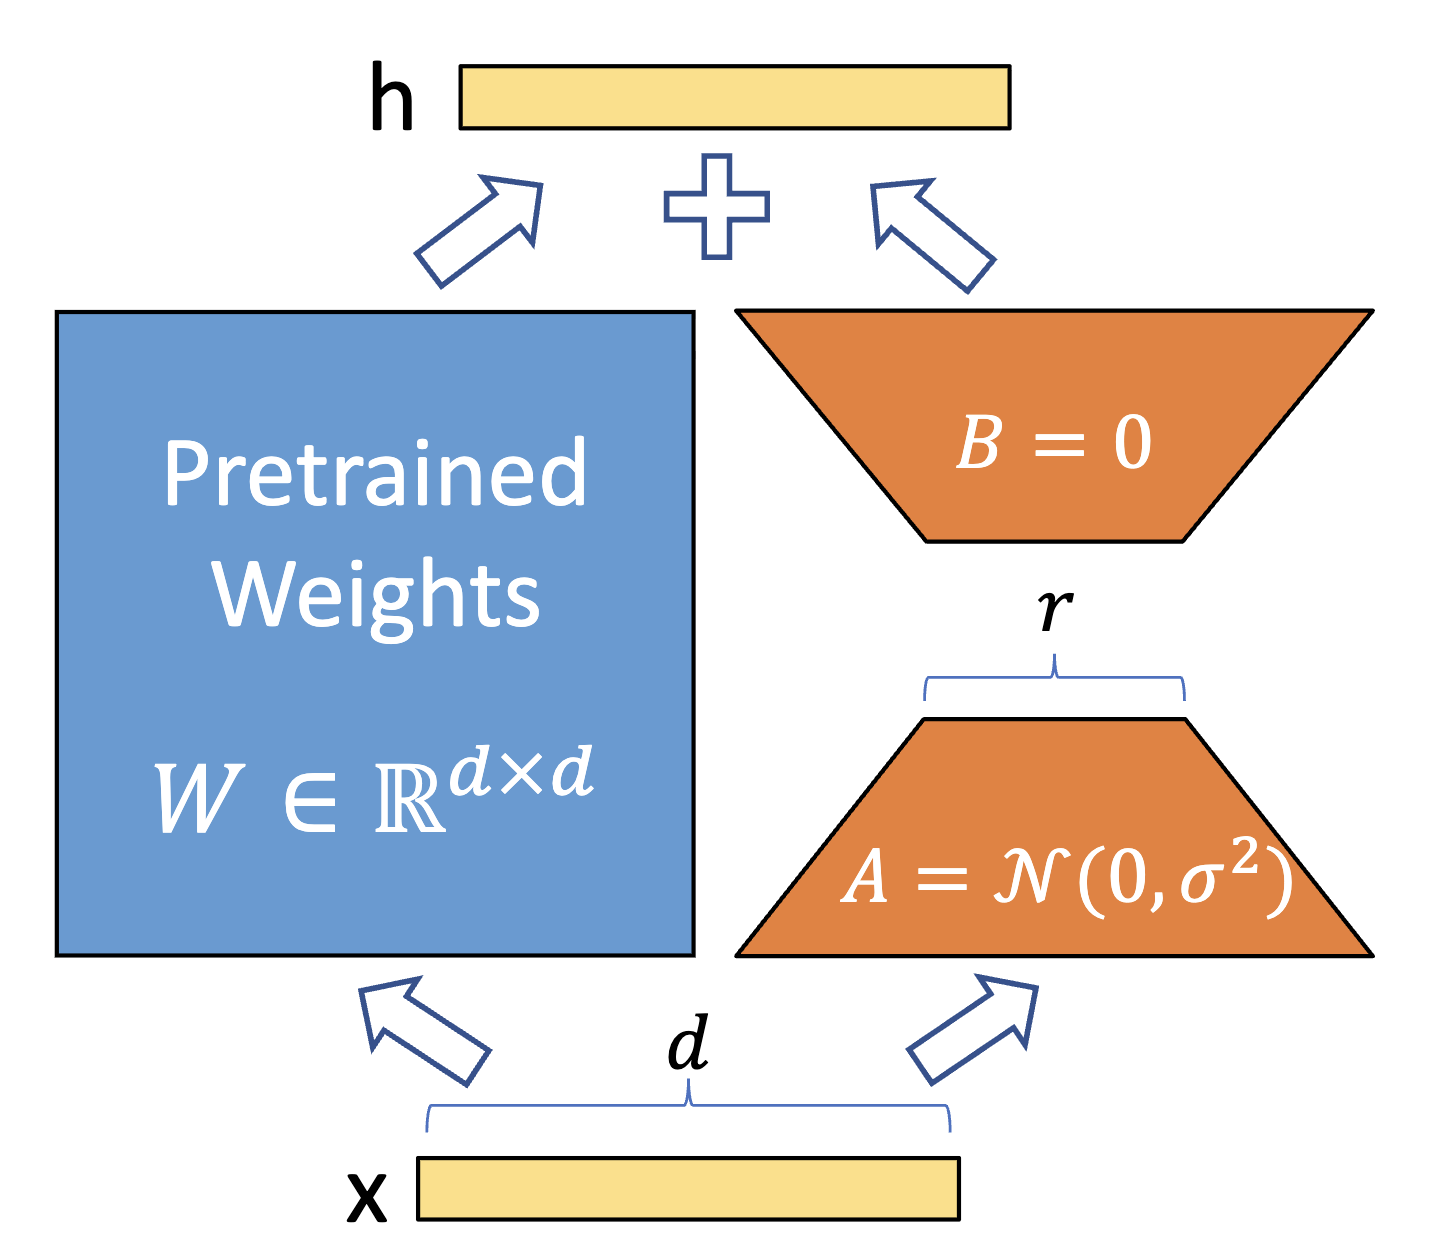
\includegraphics[width=0.6\columnwidth]{img/lora_architecture.png}
    \caption{Conceptual diagram of Parameter-Efficient Fine-Tuning (PEFT). The frozen pre-trained weights are bypassed by trainable low-rank matrices (LoRA) or parallel bottleneck modules (AdaptFormer).}
    \label{fig:peft_architecture}
\end{figure}
\section{Methodology}
\label{sec:method}

Our approach to establishing pixel-accurate semantic correspondences is structured into four progressive stages, leveraging the rich internal representations of Visual Foundation Models (VFMs).

\subsection{Phase 1: Training-Free Baseline}
The baseline relies entirely on the frozen latent representations of pre-trained backbones (DINOv2, DINOv3, and SAM) without gradient updates. For a given pair of source and target images, dense feature maps are extracted. To match a specific source keypoint, we compute the cosine similarity between its corresponding feature vector and all patch features in the target image. The predicted match is obtained using a standard, non-differentiable \textit{argmax} operator on the resulting similarity map. To ensure precise alignment, images are resized to a fixed resolution — $518\times518$ for DINOv2 (37 patches of size 14) and $512\times512$ for DINOv3 and SAM (32 patches of size 16). SAM additionally upsamples internally to $1024\times1024$ before encoding; keypoint coordinates are mapped back to the $512\times512$ frame.

\subsection{Phase 2: Light Fine-Tuning}
To improve domain adaptation and correspondence accuracy, we perform supervised fine-tuning by unfreezing only the final layers of the vision encoders, keeping early representation layers frozen. We optimize the network using a Gaussian Cross-Entropy loss. Instead of penalizing all non-exact pixel predictions equally, this loss relaxes the ground truth point into a 2D Gaussian probability distribution, computing the cross-entropy against the predicted softmax probability map. This formulation accounts for the inherent ambiguity in dense matching.

\subsection{Phase 3: Inference Refinement}
The standard \textit{argmax} operation locks predictions to discrete patch centers and is highly sensitive to local noise peaks. To achieve sub-pixel accuracy at inference time, we replace it with the Windowed Soft-Argmax (WSA). As illustrated in Figure~\ref{fig:wsa_pipeline}, WSA first identifies the coarse peak via \textit{argmax}, instantiates a small fixed window (e.g., $5 \times 5$) around this peak, and applies a soft-argmax operation exclusively within this local region. This step is applied solely during evaluation and does not affect the training objective.

\begin{figure}[ht]
    \centering
    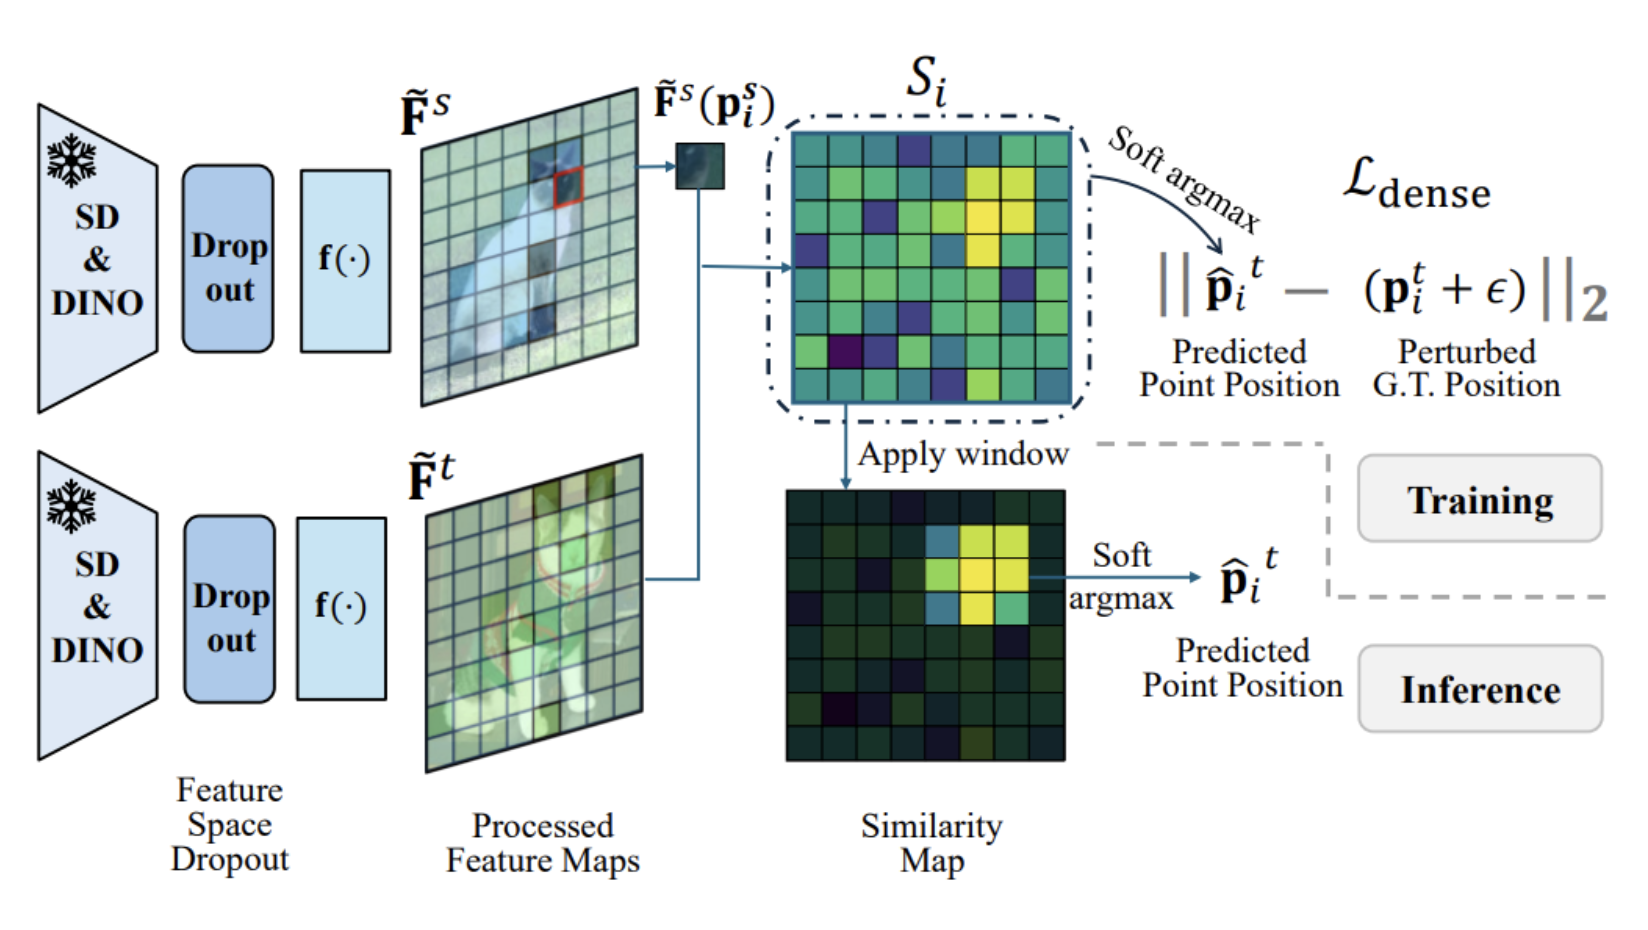
\includegraphics[width=\columnwidth]{img/wsa_pipeline.png}
    \caption{Overview of the dense matching pipeline and Inference Refinement. The similarity map is processed using a Windowed Soft-Argmax to achieve robust, sub-pixel accurate keypoint predictions.}
    \label{fig:wsa_pipeline}
\end{figure}

\subsection{Phase 4: Extensions (Parameter-Efficient Fine-Tuning)}
As an advanced exploration, we implemented a Parameter-Efficient Fine-Tuning (PEFT) strategy using Low-Rank Adaptation (LoRA). Full fine-tuning of massive vision backbones is computationally expensive and memory-intensive. To mitigate this, LoRA freezes the pre-trained model weights and injects trainable rank-decomposition matrices into the network. 

In our implementation, we applied manual LoRA adapters exclusively to the Multilayer Perceptron (MLP) linear layers of the final Transformer blocks. This surgical intervention drastically reduces the number of trainable parameters while giving the model enough flexibility to adapt to the semantic correspondence task on the SPair-71k dataset.
\section{Experiments}
\label{sec:experiments}

\subsection{Experimental Setup}
\paragraph{Dataset and Metrics.} We evaluate our models on the SPair-71k benchmark~\cite{min2019spair}. Following strict validation protocols, the training split is used for optimization, the validation split for hyperparameter tuning, and the test split exclusively for final reporting. Performance is measured using the Percentage of Correct Keypoints (PCK) metric at thresholds $\alpha \in \{0.05, 0.1, 0.2\}$, normalized by the target object's bounding box size.

\paragraph{Implementation Details.} Experiments are conducted using the Base (ViT-B) variants of DINOv2, DINOv3, and SAM. Both fine-tuning and LoRA stages are trained with AdamW on a Gaussian Cross-Entropy loss. Fine-tuning uses LR $5\times10^{-5}$ and weight decay $0.01$; LoRA uses LR $10^{-3}$ and weight decay $0.0$ (no regularization, as the low-rank matrices are already strongly constrained by their rank). Due to memory constraints, the batch size is set to 20 for DINO backbones and 4 for SAM. Input images are resized to fixed resolutions: $518\times518$ for DINOv2 and $512\times512$ for DINOv3 and SAM. Training uses early stopping with patience 7 on validation loss. LoRA adapters (rank 8, $\alpha{=}16$) are applied to the MLP layers of the last $N$ transformer blocks, where $N$ is swept over $\{1, 2, 4\}$ as an ablation (Section~\ref{sec:ablations}). For fine-tuning, we additionally run a no-augmentation variant to quantify the effect of photometric data augmentation. Throughput (images/sec) and peak GPU memory are measured after three warm-up batches to characterize computational efficiency.
All experiments were conducted on a dedicated virtual machine hosted on a Proxmox hypervisor, equipped with an NVIDIA GeForce RTX~5080 GPU (16\,GB VRAM), an Intel Core i5 processor with 10 logical cores allocated out of 20 available on the host, and 24\,GB of RAM out of 32\,GB available on the host system. Training the full pipeline (18 fine-tuning and LoRA stages across three backbones and three adaptation depths) required several days of uninterrupted GPU computation, making repeated full re-runs for hyperparameter search infeasible within the project timeline.

\subsection{Quantitative Results}
Table~\ref{tab:quantitative_results} summarizes the PCK performance of all evaluated backbones across methodological stages. Per-image (macro) PCK is reported; per-keypoint (micro) results are provided in the supplementary material. All values are measured on the SPair-71k test split.
\TODO{Fill in all PCK values in Table~\ref{tab:quantitative_results} from \texttt{runs/pipeline\_exports/pck\_results.csv} after pipeline execution. Bold the column-wise best per section. The master table is auto-generated by AML\_Analysis.ipynb §B.}

\begin{table}[ht]
    \centering
    \caption{PCK evaluation on the SPair-71k test split (per-image macro). Best result in each column is in \textbf{bold}. WSA = Windowed Soft-Argmax; FT = Fine-Tuned last $N$ blocks.}
    \label{tab:quantitative_results}
    \resizebox{\columnwidth}{!}{%
    \begin{tabular}{llcccc}
        \toprule
        \textbf{Model} & \textbf{Method} & \textbf{Blocks} & \textbf{PCK@0.05} & \textbf{PCK@0.10} & \textbf{PCK@0.20} \\
        \midrule
        \multicolumn{6}{l}{\textit{Training-Free Baseline}} \\
        DINOv2 (ViT-B) & Baseline (Argmax) & —  & — & — & — \\
        DINOv2 (ViT-B) & Baseline + WSA    & —  & — & — & — \\
        DINOv3 (ViT-B) & Baseline (Argmax) & —  & — & — & — \\
        DINOv3 (ViT-B) & Baseline + WSA    & —  & — & — & — \\
        SAM    (ViT-B) & Baseline (Argmax) & —  & — & — & — \\
        SAM    (ViT-B) & Baseline + WSA    & —  & — & — & — \\
        \midrule
        \multicolumn{6}{l}{\textit{Light Fine-Tuning (last $N$ blocks)}} \\
        DINOv2 (ViT-B) & FT (Argmax) & 1 & — & — & — \\
        DINOv2 (ViT-B) & FT + WSA    & 1 & — & — & — \\
        DINOv2 (ViT-B) & FT (Argmax) & 2 & — & — & — \\
        DINOv2 (ViT-B) & FT + WSA    & 2 & — & — & — \\
        DINOv2 (ViT-B) & FT (Argmax) & 4 & — & — & — \\
        DINOv2 (ViT-B) & FT + WSA    & 4 & — & — & — \\
        DINOv3 (ViT-B) & FT (Argmax) & 1 & — & — & — \\
        DINOv3 (ViT-B) & FT + WSA    & 1 & — & — & — \\
        DINOv3 (ViT-B) & FT (Argmax) & 2 & — & — & — \\
        DINOv3 (ViT-B) & FT + WSA    & 2 & — & — & — \\
        DINOv3 (ViT-B) & FT (Argmax) & 4 & — & — & — \\
        DINOv3 (ViT-B) & FT + WSA    & 4 & — & — & — \\
        SAM    (ViT-B) & FT (Argmax) & 1 & — & — & — \\
        SAM    (ViT-B) & FT + WSA    & 1 & — & — & — \\
        SAM    (ViT-B) & FT (Argmax) & 2 & — & — & — \\
        SAM    (ViT-B) & FT + WSA    & 2 & — & — & — \\
        SAM    (ViT-B) & FT (Argmax) & 4 & — & — & — \\
        SAM    (ViT-B) & FT + WSA    & 4 & — & — & — \\
        \midrule
        \multicolumn{6}{l}{\textit{LoRA (rank 8, $\alpha{=}16$, last $N$ blocks)}} \\
        DINOv2 (ViT-B) & LoRA (Argmax) & 1 & — & — & — \\
        DINOv2 (ViT-B) & LoRA + WSA    & 1 & — & — & — \\
        DINOv2 (ViT-B) & LoRA (Argmax) & 2 & — & — & — \\
        DINOv2 (ViT-B) & LoRA + WSA    & 2 & — & — & — \\
        DINOv2 (ViT-B) & LoRA (Argmax) & 4 & — & — & — \\
        DINOv2 (ViT-B) & LoRA + WSA    & 4 & — & — & — \\
        DINOv3 (ViT-B) & LoRA (Argmax) & 1 & — & — & — \\
        DINOv3 (ViT-B) & LoRA + WSA    & 1 & — & — & — \\
        DINOv3 (ViT-B) & LoRA (Argmax) & 2 & — & — & — \\
        DINOv3 (ViT-B) & LoRA + WSA    & 2 & — & — & — \\
        DINOv3 (ViT-B) & LoRA (Argmax) & 4 & — & — & — \\
        DINOv3 (ViT-B) & LoRA + WSA    & 4 & — & — & — \\
        SAM    (ViT-B) & LoRA (Argmax) & 1 & — & — & — \\
        SAM    (ViT-B) & LoRA + WSA    & 1 & — & — & — \\
        SAM    (ViT-B) & LoRA (Argmax) & 2 & — & — & — \\
        SAM    (ViT-B) & LoRA + WSA    & 2 & — & — & — \\
        SAM    (ViT-B) & LoRA (Argmax) & 4 & — & — & — \\
        SAM    (ViT-B) & LoRA + WSA    & 4 & — & — & — \\
        \bottomrule
    \end{tabular}
    }
\end{table}

\subsection{Qualitative Results}
Visualizing predictions provides critical insights into the models' geometric and semantic awareness. Figure~\ref{fig:qualitative} compares the standard argmax predictions with the WSA refined outputs, highlighting cases where standard argmax suffers from local noise or symmetry ambiguity.

\TODO{Replace placeholder image with the method-comparison grid generated by AML\_Analysis.ipynb §G (\texttt{runs/paper\_figures/qualitative/}). Use a grid showing source image, target image, argmax prediction vs.\ WSA prediction vs.\ ground truth for representative pairs. Include at least one failure case (symmetry ambiguity).}

\begin{figure}[H]
    \centering
    
\includegraphics[width=\columnwidth]{img/qualitative_results.png}
    \caption{Qualitative comparison of semantic matching. Green dots denote ground truth, red crosses denote baseline predictions, and yellow stars denote WSA-refined predictions.}
    \label{fig:qualitative}
\end{figure}

\subsection{Ablation Studies}
\label{sec:ablations}

\paragraph{WSA Window Size.}
To quantify the sensitivity of Windowed Soft-Argmax to the window hyperparameter, we sweep over window sizes $w \in \{3, 5, 7, 9\}$ on the frozen baseline (no fine-tuning). The argmax location is fixed; only the local soft-argmax region changes. Results are reported at PCK@0.10.
\TODO{Insert WSA window sensitivity figure from AML\_Analysis.ipynb §C.4 (\texttt{runs/paper\_figures/figures/wsa\_window\_sensitivity\_a0.1.pdf}). Discuss the optimal window and sensitivity to this hyperparameter.}

\paragraph{DINO Intermediate Layer.}
Terminal ViT layers aggregate global classification information, which can reduce spatial granularity useful for dense matching. We evaluate feature extraction from intermediate layers $l \in \{4, 9, 11\}$ (out of 12) on the frozen DINOv2 and DINOv3 baselines to identify which depth provides the best trade-off between semantic abstraction and geometric precision.
\TODO{Insert DINO layer sensitivity figure from AML\_Analysis.ipynb §C.4 (\texttt{runs/paper\_figures/figures/dino\_layer\_sensitivity\_a0.1.pdf}). Report which layer index maximises PCK@0.10 for each backbone.}

\paragraph{Fine-Tuning Depth.}
The number of unfrozen transformer blocks ($N \in \{1, 2, 4\}$) controls the adaptation capacity. We analyze how PCK evolves with fine-tuning depth across all three backbones, measuring the trade-off between added trainable parameters and correspondence quality.
\TODO{Insert fine-tuning depth figure from AML\_Analysis.ipynb §C.2 (\texttt{runs/paper\_figures/figures/ft\_depth.pdf}). Discuss the sweet spot between frozen and fully fine-tuned configurations.}

\paragraph{LoRA Depth.}
Analogously to the fine-tuning depth ablation, we sweep the number of LoRA-equipped blocks over $N \in \{1, 2, 4\}$ for each backbone. This isolates the contribution of adaptation depth from the parameter budget, as rank and $\alpha$ are kept fixed.
\TODO{Insert LoRA depth figure from AML\_Analysis.ipynb (\texttt{runs/paper\_figures/figures/lora\_depth.pdf}). Report whether the LoRA depth trend mirrors the fine-tuning depth trend, and identify the optimal $N$ per backbone.}

\paragraph{Photometric Augmentation.}
To measure the regularization benefit of photometric data augmentation during fine-tuning, we run each fine-tuning configuration (backbone $\times$ block count) a second time with augmentation disabled. The no-augmentation variant uses identical hyperparameters and the same early-stopping criterion.
\TODO{Insert augmentation ablation figure from AML\_Analysis.ipynb (\texttt{runs/paper\_figures/figures/aug\_ablation.pdf}). Report the average $\Delta$PCK@0.10 attributable to augmentation and whether its benefit is uniform across backbones and block counts.}

\paragraph{Computational Efficiency.}
We evaluate the computational cost of each configuration by measuring inference throughput (images/sec) and peak GPU memory allocation. Throughput is estimated over 10 batches after a 3-batch warm-up to exclude GPU initialization overhead. This allows direct comparison of the accuracy--efficiency trade-off across backbone size, method, and adaptation depth.
\TODO{Insert efficiency scatter plot from AML\_Analysis.ipynb (\texttt{runs/paper\_figures/figures/efficiency\_scatter.pdf}). Report peak memory and throughput for baseline, best FT, and best LoRA configurations. Cite \texttt{runs/pipeline\_exports/efficiency\_results.json} for exact values.}
\section{Discussion}
\label{sec:discussion}

The experimental results yield several key insights regarding the capabilities and limitations of Visual Foundation Models (VFMs) in dense semantic matching tasks.

\paragraph{Backbone Comparison: Semantic vs. Structural Awareness.}
Our evaluation highlights a clear distinction in how different backbones encode visual information. The DINO family (DINOv2 and DINOv3) demonstrates superior semantic abstraction, accurately linking object parts even across significant domain shifts (e.g., photos to paintings). Conversely, the Segment Anything Model (SAM) exhibits exceptionally strong structural and boundary awareness due to its mask-based pre-training. However, SAM's class-agnostic nature occasionally leads to geometrically precise but semantically incorrect matches compared to DINO.
\TODO{Add quantitative backbone comparison: report best PCK@0.10 per backbone at baseline, citing specific values from Table~\ref{tab:quantitative_results}. Mention which backbone achieves the highest zero-shot PCK and whether the ranking holds after fine-tuning.}

\paragraph{Impact of Inference Refinement.}
The transition from a standard discrete \textit{argmax} to the Windowed Soft-Argmax (WSA) systematically improved the Percentage of Correct Keypoints (PCK) across all precision thresholds. By enabling sub-pixel coordinate prediction, WSA effectively mitigates the discretization error inherent in patch-based ViT architectures and reduces the model's sensitivity to isolated noise spikes in the similarity maps.
\TODO{Quantify the average WSA gain ($\Delta$PCK@0.10) across all backbones and stages from \texttt{runs/paper\_figures/figures/wsa\_gain\_a0.1.pdf}. Discuss whether WSA gain is larger on the frozen baseline or on fine-tuned models.}

\paragraph{Efficiency of Low-Rank Adaptation.}
Full fine-tuning of large-scale ViT backbones is highly inefficient. The implementation of LoRA on the Multilayer Perceptron (MLP) layers of the final Transformer blocks proved to be a highly effective compromise: it significantly reduces the number of trainable parameters and memory footprint while providing sufficient capacity to adapt the frozen zero-shot features to the geometric nuances of the SPair-71k benchmark. Our LoRA depth sweep ($N \in \{1,2,4\}$) further characterizes how adaptation depth interacts with parameter efficiency, enabling a fine-grained accuracy–cost trade-off analysis. Measured inference throughput and peak GPU memory (reported in \texttt{efficiency\_results.json}) allow direct comparison of all configurations on the same hardware.
\TODO{Report exact trainable parameter counts (from AML\_Analysis.ipynb §H, \texttt{runs/paper\_figures/tables/efficiency.csv}): how many parameters does LoRA add vs.\ full fine-tuning of the last $N$ blocks? Report the PCK@0.10 gap between LoRA and the best FT configuration, and the throughput ratio between the most and least efficient configurations.}

\paragraph{Effect of Photometric Augmentation.}
The augmentation ablation (Section~\ref{sec:ablations}) isolates the contribution of photometric transformations applied during fine-tuning. Augmentation is expected to improve generalization particularly for backbones that are already strongly pretrained, where fine-tuning with clean data can lead to feature collapse on the training distribution.
\TODO{Quantify the average $\Delta$PCK@0.10 attributable to augmentation across all backbone $\times$ block configurations. Discuss whether the benefit is consistent or backbone-specific, referencing \texttt{runs/paper\_figures/figures/aug\_ablation.pdf}.}

\paragraph{Limitations and Failure Cases.}
Despite the improvements, semantic correspondence remains challenging under extreme conditions. Qualitative analysis reveals that the models still struggle with severe truncations and symmetry ambiguity (e.g., consistently distinguishing a left eye from a right eye when the object undergoes a severe out-of-plane rotation). Addressing these geometry-aware semantic failures remains an open challenge for future work.
\TODO{Add per-difficulty breakdown (viewpoint / scale / truncation / occlusion) from AML\_Analysis.ipynb §E (\texttt{runs/paper\_figures/tables/per\_difficulty\_a0.1.csv}). Identify which difficulty factor causes the largest PCK drop. Add per-category heatmap figure from §D if space allows.}
\section{Conclusion}
\label{sec:conclusion}

This project presented a comprehensive evaluation of Visual Foundation Models (VFMs) for the challenging task of pixel-level semantic correspondence. By systematically analyzing DINOv2, DINOv3, and SAM on the SPair-71k benchmark, we established key insights into the trade-offs between zero-shot semantic abstraction and fine-tuned geometric accuracy.

Our progressive experimental pipeline demonstrated that:
\begin{itemize}
    \item \textbf{VFMs as Dense Extractors:} Pre-trained vision backbones provide strong zero-shot baselines, though they inherently differ in their balance of semantic versus structural awareness.
    \item \textbf{Inference Refinement is Crucial:} The integration of Windowed Soft-Argmax (WSA) effectively resolves discretization errors and mitigates local noise, consistently improving PCK metrics across all tested models.
    \item \textbf{Parameter-Efficient Adaptation:} Low-Rank Adaptation (LoRA) applied exclusively to the final MLP blocks offers a highly efficient strategy to adapt massive vision backbones to specific geometric downstream tasks. Our depth sweep ($N \in \{1,2,4\}$ LoRA blocks) shows that even a single adapted block yields meaningful gains, with diminishing returns beyond a backbone-specific optimum.
    \item \textbf{Augmentation as Regularizer:} Photometric augmentation during fine-tuning provides a consistent PCK improvement, with the effect being most pronounced for backbones that are less expressive at the block counts considered.
\end{itemize}

\TODO{Update the bullet points above with actual quantitative claims once results are available (e.g., ``improving PCK@0.10 by $+X.X\%$ on average'', ``achieving $Y\%$ PCK@0.10 with only $Z$K trainable parameters'', ``augmentation contributes $+\Delta\%$ PCK@0.10 on average''). Values come from Table~\ref{tab:quantitative_results}, \texttt{runs/paper\_figures/tables/efficiency.csv}, and \texttt{runs/paper\_figures/figures/aug\_ablation.pdf}.}

While significant improvements were achieved through fine-tuning and inference refinement, establishing flawless semantic correspondence under extreme viewpoint variations and symmetry ambiguities remains an open problem. Future research directions may explore the integration of diffusion-based geometry-aware features or extend the evaluation to cross-domain datasets to further validate the generalization capabilities of these foundational representations.

{
    \small
    \bibliographystyle{ieeenat_fullname}
    \bibliography{main}
}

\section*{Supplementary Material}

\subsection*{Per-Keypoint (Micro) PCK Results}
\label{sec:supp_micro}

Table~\ref{tab:micro_pck} reports per-keypoint (micro) PCK on the SPair-71k test split, complementing the per-image (macro) results in Table~\ref{tab:quantitative_results}. Micro PCK weights each keypoint equally regardless of how many annotated points an image contains, making it more sensitive to frequently occurring keypoints (e.g., eyes, wheels) than macro PCK.

\TODO{Fill all values in Table~\ref{tab:micro_pck} from \texttt{runs/pipeline\_exports/pck\_results.csv} (column \texttt{pck\_per\_point@\{0.05,0.10,0.20\}}). The master table is auto-generated by AML\_Analysis.ipynb §B.}

\begin{table}[ht]
    \centering
    \caption{Per-keypoint (micro) PCK on the SPair-71k test split. WSA = Windowed Soft-Argmax; FT = Fine-Tuned last $N$ blocks.}
    \label{tab:micro_pck}
    \resizebox{\columnwidth}{!}{%
    \begin{tabular}{llcccc}
        \toprule
        \textbf{Model} & \textbf{Method} & \textbf{Blocks} & \textbf{PCK@0.05} & \textbf{PCK@0.10} & \textbf{PCK@0.20} \\
        \midrule
        \multicolumn{6}{l}{\textit{Training-Free Baseline}} \\
        DINOv2 (ViT-B) & Baseline (Argmax) & — & — & — & — \\
        DINOv2 (ViT-B) & Baseline + WSA    & — & — & — & — \\
        DINOv3 (ViT-B) & Baseline (Argmax) & — & — & — & — \\
        DINOv3 (ViT-B) & Baseline + WSA    & — & — & — & — \\
        SAM    (ViT-B) & Baseline (Argmax) & — & — & — & — \\
        SAM    (ViT-B) & Baseline + WSA    & — & — & — & — \\
        \midrule
        \multicolumn{6}{l}{\textit{Light Fine-Tuning (last $N$ blocks)}} \\
        DINOv2 (ViT-B) & FT (Argmax) & 1 & — & — & — \\
        DINOv2 (ViT-B) & FT + WSA    & 1 & — & — & — \\
        DINOv2 (ViT-B) & FT (Argmax) & 2 & — & — & — \\
        DINOv2 (ViT-B) & FT + WSA    & 2 & — & — & — \\
        DINOv2 (ViT-B) & FT (Argmax) & 4 & — & — & — \\
        DINOv2 (ViT-B) & FT + WSA    & 4 & — & — & — \\
        DINOv3 (ViT-B) & FT (Argmax) & 1 & — & — & — \\
        DINOv3 (ViT-B) & FT + WSA    & 1 & — & — & — \\
        DINOv3 (ViT-B) & FT (Argmax) & 2 & — & — & — \\
        DINOv3 (ViT-B) & FT + WSA    & 2 & — & — & — \\
        DINOv3 (ViT-B) & FT (Argmax) & 4 & — & — & — \\
        DINOv3 (ViT-B) & FT + WSA    & 4 & — & — & — \\
        SAM    (ViT-B) & FT (Argmax) & 1 & — & — & — \\
        SAM    (ViT-B) & FT + WSA    & 1 & — & — & — \\
        SAM    (ViT-B) & FT (Argmax) & 2 & — & — & — \\
        SAM    (ViT-B) & FT + WSA    & 2 & — & — & — \\
        SAM    (ViT-B) & FT (Argmax) & 4 & — & — & — \\
        SAM    (ViT-B) & FT + WSA    & 4 & — & — & — \\
        \midrule
        \multicolumn{6}{l}{\textit{LoRA (rank 8, $\alpha{=}16$, last $N$ blocks)}} \\
        DINOv2 (ViT-B) & LoRA (Argmax) & 1 & — & — & — \\
        DINOv2 (ViT-B) & LoRA + WSA    & 1 & — & — & — \\
        DINOv2 (ViT-B) & LoRA (Argmax) & 2 & — & — & — \\
        DINOv2 (ViT-B) & LoRA + WSA    & 2 & — & — & — \\
        DINOv2 (ViT-B) & LoRA (Argmax) & 4 & — & — & — \\
        DINOv2 (ViT-B) & LoRA + WSA    & 4 & — & — & — \\
        DINOv3 (ViT-B) & LoRA (Argmax) & 1 & — & — & — \\
        DINOv3 (ViT-B) & LoRA + WSA    & 1 & — & — & — \\
        DINOv3 (ViT-B) & LoRA (Argmax) & 2 & — & — & — \\
        DINOv3 (ViT-B) & LoRA + WSA    & 2 & — & — & — \\
        DINOv3 (ViT-B) & LoRA (Argmax) & 4 & — & — & — \\
        DINOv3 (ViT-B) & LoRA + WSA    & 4 & — & — & — \\
        SAM    (ViT-B) & LoRA (Argmax) & 1 & — & — & — \\
        SAM    (ViT-B) & LoRA + WSA    & 1 & — & — & — \\
        SAM    (ViT-B) & LoRA (Argmax) & 2 & — & — & — \\
        SAM    (ViT-B) & LoRA + WSA    & 2 & — & — & — \\
        SAM    (ViT-B) & LoRA (Argmax) & 4 & — & — & — \\
        SAM    (ViT-B) & LoRA + WSA    & 4 & — & — & — \\
        \bottomrule
    \end{tabular}
    }
\end{table}

\subsection*{GitHub Repository}
\label{sec:repo}

\url{https://github.com/lucaosti/Semantic-Correspondence}


\end{document}
